\documentclass[12pt,compress,aspectratio=169]{beamer}
\usetheme{metropolis}
\setbeamersize{text margin left=.5cm,text margin right=.5cm}
\usepackage[lf]{carlito}
\usepackage{siunitx}
\usepackage{tikz}
\usepackage{mathpazo}
\usepackage{bm}
\usepackage{mathtools}
\usepackage[ISO]{diffcoeff}
\diffdef{}{ op-symbol=\mathsf{d} }
\usepackage{xcolor,colortbl}

\setmonofont{Ubuntu Mono}
\setlength{\parskip}{0pt}
\renewcommand{\baselinestretch}{1}

\sisetup{
  inter-unit-product=\cdot,
  per-mode=symbol
}

\tikzset{
  >=latex
}

%\newcommand{\iii}{\hat{\bm\imath}}
%\newcommand{\jjj}{\hat{\bm\jmath}}
%\newcommand{\kkk}{\hat{\bm k}}

\usepackage{mathtools}
  
\sisetup{
  per-mode=symbol
}
\tikzset{>=latex}

\setmonofont{Ubuntu Mono}
\setlength{\parskip}{0pt}
\renewcommand{\baselinestretch}{1}


\title{Topic 1: Kinematics}
\subtitle{Advanced Placement Physics C}
\author[TML]{Dr.\ Timothy Leung}
\institute{Olympiads School}
\date{Updated: Summer 2022}


\newcommand{\iii}{\ensuremath\hat{\bm{\imath}}}
\newcommand{\jjj}{\ensuremath\hat{\bm{\jmath}}}
\newcommand{\kkk}{\ensuremath\hat{\bm{k}}}
\newcommand{\eq}[2]{\vspace{#1}{\Large\begin{displaymath}#2\end{displaymath}}}



\begin{document}

\begin{frame}{}

  {\LARGE
    \begin{center}
      \textbf{WELCOME TO AP PHYSICS C}
    \end{center}
  }
\end{frame}



%\begin{frame}{Prerequisites}
%  \begin{itemize}
%  \item\textbf{Physics 11 and 12:} You will need to be comfortable with the
%    topics covered in high-school level physics courses.
%  \item\textbf{Calculus:} Physics C exams are calculus based, and you will be
%    required to do basic differentiation and integration. You don't need to be
%    an expert, but basic knowledge is required. Differentiation and integration
%    in the course are generally not difficult, but there are occasional
%    challenges.
%  \item\textbf{Vectors:} You need to be comfortable with vector operations,
%    including addition and subtraction, multiplication/division by constants,
%    as well as dot products and cross products.
%  \end{itemize}
%\end{frame}



\begin{frame}{AP Physics C Exams}
  There are two calculus-based AP Physics C exams, which are usually taken
  together on the same day, in the first or second week of May of each year.
  \begin{itemize}
  \item Mechanics
  \item Electricity and Magnetism
  \end{itemize}
\end{frame}



\begin{frame}
  \titlepage
\end{frame}



\begin{frame}{Files for You to Download}
  There are a considerable number of files for you to download at the beginning
  of the course:
  \begin{itemize}
  \item\texttt{PhysAPC-courseOutline.pdf}--The course outline
  \item\texttt{PhysAPC-equationSheet.pdf}--Equation sheet for your exams
  \item\texttt{PhysAPC-01-kinematics.pdf}
  \item\texttt{PhysAPC-01a-vectorCalculus.pdf}--Vectors and calculus handout
  \item\texttt{PhysAPC-01b-kinematicsHandout.pdf}--Basic kinematics, expanded
    version
  %\item\texttt{PhysAPC-01c-motionGraphs.pdf}--Handout on motion graphs
  \item\texttt{PhysAPC-01d-projectileMotion.pdf}--Handout on projectile motion
  %\item\texttt{PhysAPC-02-dynamics.pdf}
  \item\texttt{PhysAPC-01-Homework.pdf}--Homework problems for Topic 1
  %\item\texttt{PhysAPC-02-Homework.pdf}--Homework problems for Topic 2
  \end{itemize}
\end{frame}


\begin{frame}{File Download}
  Please download/print the PDF file for the class slides before
  each class. There is no point copying notes that are already on the slides.
  Instead, focus on things that aren't necessarily on the slides. If you wish
  to print the slides, we recommend printing \emph{four} slides per page.
\end{frame}



\begin{frame}{Vectors and Calculus}
  Please refer to the handout to make sure that you are familiar with
  basic vector and calculus.
\end{frame}



\section{Kinematics}

%\begin{frame}{Kinematics}
%  \textbf{Kinematics} is a discipline within mechanics concerning the
%  motion of bodies. It describes the mathematical relationship between 
%  \begin{itemize}
%  \item<alert@1> Position
%  \item<alert@1> Displacement
%  \item Distance 
%  \item<alert@1> Velocity
%  \item Speed
%  \item<alert@1> Acceleration
%  \end{itemize}
%  Kinematics does not deal with the causes of motion. The quantities that are
%  highlighted are vectors.
%\end{frame}



\begin{frame}{Position}
  \textbf{Position} ($\bm{x}(t)$) describes the location of an object in a
  predefined coordinate system. %The origin of
  %\footnote{The coordinate system is usually
  %\emph{Cartesian}, but it can also be \emph{polar}, \emph{cylindrical} or
  %\emph{spherical}}.
  %the coordinate system is called the ``reference point''.
  %The SI unit for position is \textbf{meter}, \si{\metre}.
  
  \eq{-.2in}{
    \boxed{\bm{x}(t)=x(t)\iii + y(t)\jjj + z(t)\kkk}
  }

  Vectors in 2D/3D Cartesian space are generally using the
  \textbf{IJK notation}
  \begin{itemize}
  \item $\iii$, $\jjj$ and $\kkk$ are \textbf{basis vectors} indicating the
    directions of the $x$, $y$ and $z$ axes. Basis vectors are
    \textbf{unit vectors} (i.e.\ length $1$)
  \item The IJK notation does not explicitly give the magnitude or the direction
    of the vector (needs to be calculated using the Pythagorean theorem)
  \end{itemize}
\end{frame}



\begin{frame}{Displacement}
  \textbf{Displacement} $\Delta\bm{x}(t)$ is the change in position from the
  initial position $\bm{x}_0$ within the same coordinate system:

  \eq{-.25in}{
    \boxed{
      \Delta\bm{x}(t)=\bm{x}(t)-\bm{x}_0
      =(x-x_0)\iii + (y-y_0)\jjj + (z-z_0)\kkk
    }
  }
  %\begin{itemize}
  %\item IJK notation makes vector addition and subtraction less prone to errors
  %\item Since the reference point $\bm{x}_\text{ref}=\bm{0}$, the position
  %  vector $\bm{x}$ is also its displacement from the reference point
  %\end{itemize}
\end{frame}



\begin{frame}{Distance}
  \textbf{Distance} $s(t)$ is a quantity that is \emph{related} to displacement.
  %The unit for distance is also a meter (\si{\metre}).
  \begin{columns}
    \column{.7\textwidth}
    \begin{itemize}
    \item The \emph{length of the path} taken by an object when it travels from
      $\bm{x}_0$ to $\bm{x}(t)$
    \item A scalar quantity
    \item Always positive, i.e.\ $s\geq 0$
    \item Although the magnitude of the displacement vector is also a scalar,
      it is not necessarily the same as distance
    \item $s\geq |\Delta\bm{x}|$
    \end{itemize}
    
    \column{.3\textwidth}
    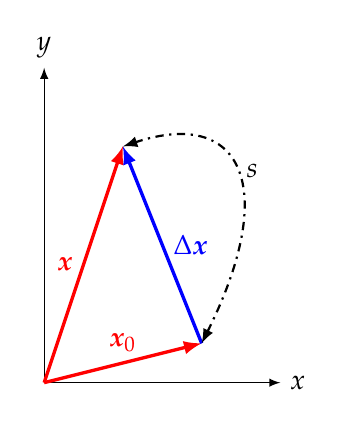
\begin{tikzpicture}[scale=.5]
      \draw[->](0,0)--(6,0) node[right]{$x$};
      \draw[->](0,0)--(0,8) node[above]{$y$};
      \draw[->,red,very thick] (0,0)--(4,1) node[midway,above]{$\bm{x}_0$};
      \draw[->,red,very thick] (0,0)--(2,6) node[midway,left]{$\bm{x}$};
      \draw[->,blue,very thick](4,1)--(2,6) node[midway,right]{$\Delta\bm{x}$};
      \draw[thick,dash dot,<->] (4,1)..controls (6,5) and (5,7)..(2,6)
      node[midway,right]{$s$};
    \end{tikzpicture}
  \end{columns}
\end{frame}



\begin{frame}{Instantaneous \& Average Velocity}
  \textbf{Instantaneous velocity} $\bm{v}(t)$ is the time rate of change in
  position. It is related to positiion $\bm{x}(t)$ by:
  %\textbf{average velocity}
%  $\overline{\bm{v}}$ are defined as:
%  %Position $\bm{x}$ is continuously differentiable in time $t$, and the
%  %\textbf{instantaneous velocity} can be found at any time by differentiating
%  %$\bm{x}$ with respect to $t$:
%  %The unit for velocity is
%  %\textbf{meters per second} (\si{\metre\per\second}):

  \eq{-.13in}{
    \boxed{
      \bm{v}(t)= \diff{\bm{x}}t
      \quad\quad
      \bm{x}(t)=\int\bm{v}(t)\dl t + \bm{x}_0
    }
  }

  The constant of integration $\bm{x}_0$ evaluated at $t=0$. Likewise, the
  \textbf{average velocity} $\overline{\bm{v}}(t)$ is the change in
  position $\Delta\bm{x}(t)$ over a finite time interval $t$:

  \eq{-.1in}{
    \boxed{
      \overline{\bm{v}}(t)=
      \frac{\Delta\bm{x}}t=
      \frac{\bm{x}(t)-\bm{x}_0}{t}=
      \frac{\int_0^t\bm{v}\dl t}{t}
    }
  }

  
  %We can integrate each component to get $\bm{x}$:  

\end{frame}




%
%
%
%\begin{frame}{Average Velocity}
%  \textbf{Average velocity} $\overline{\bm{v}}$ of an object is the
%  \emph{finite} change in position $\Delta\bm{x}$ over a \emph{finite} time
%  interval $\Delta t$:
%
%  \eq{-.3in}{

%  }
%  
%  Like instantaneous velocity, we can find the $x$, $y$ and $z$ components of
%  average velocity by separating components in each direction:
%
%  \eq{-.15in}{
%    \overline{\bm{v}}=
%    \frac{\Delta x}{\Delta t}\iii+
%    \frac{\Delta y}{\Delta t}\jjj+
%    \frac{\Delta z}{\Delta t}\kkk
%  }
%%  The notation $\overline{v}$ means that $v$ is averaged over \emph{time},
%%  while the notation $\langle v\rangle$ is used if $v$ is the average of
%%  many particles (called an \emph{ensemble average})
%\end{frame}



\begin{frame}{Instantaneous \& Average Speed}
  \textbf{Instantaneous speed} $v$ is the time rate of change of
  \emph{distance}. It is the \emph{magnitude} of instantaneous velocity
  (i.e.\ $v=|\bm{v}|$)

  \eq{-.2in}{
    \boxed{
      v=\diff st
    }
  }

  Since $s\geq 0$, instantaneous speed must also be positive, i.e.\ $v\geq 0$.
  \textbf{Average speed} $\overline{v}(t)$ is the distance $s(t)$ travelled
  over a finite time interval $t$:
  
  \eq{-.15in}{
    \boxed{
      \overline{v}=\frac{s(t)}t=\frac{\int_0^t v\dl t}t
    }
  }
  %The SI unit of speed is also meters per second \si{\metre\per\second}.
\end{frame}



%\begin{frame}{Path}
%  Sometimes instead of explicitly describing the position $x=x(t)$ and $y=y(t)$,
%  the path of an object can be given in terms of $x$ coordinate $y=y(x)$, while
%  giving the $x$ (or $y$) coordinate as a function of time.
%  \begin{itemize}
%  \item In this case, substitute the expression for $x(t)$ into $y=y(x)$ to
%    get an expression of $y=y(t)$
%  \item Take derivative using chain rule to get $v_y=v_y(t)$
%  \end{itemize}
%\end{frame}


\begin{frame}{Instantaneous \& Average Acceleration}
  In the same way that velocity is the time rate of change in position,
  \textbf{instantaneous acceleration} $\bm{a}(t)$ is related to
  instantaneous velocity by:
  %with a unit of \textbf{meters per second squared}
  %(\si{\metre\per\second\squared}):

  \eq{-.2in}{
    \boxed{
      \bm{a}(t)= \diff{\bm{v}}t=\diff[2]{\bm{x}}t
      \quad\quad
      \bm{v}(t)=\int\bm{a}(t)\dl t+\bm{v}_0
    }
  }

  Likewise, \textbf{average acceleration} $\overline{\bm{a}}(t)$ is the finite
  change in velocity $\Delta\bm{v}(t)$ over a finite time interval $t$:

  \eq{-.27in}{
    \boxed{
      \overline{\bm{a}}(t)=
      \frac{\Delta\bm{v}(t)}t
      =\frac{\bm{v}(t)-\bm{v}_0}t
      =\frac{\int_0^t\bm{a}\dl t}t
    }
  }

  Note that acceleration only requires a \emph{change} in velocity. It does
  \emph{not} necessarily mean an object speeds up or slows down (e.g.\ uniform
  circular motion).
\end{frame}



\begin{frame}{Special Notation When Differentiating With Time}
  Physicists and engineers use a special notation when the derivative is
  taken with respect to \emph{time}, by writing a dot above the variable. For
  example:

  \vspace{-.3in}{\Large
    \begin{align*}
      \bm{v} &= \dot{\bm{x}}\\
      \bm{a} &= \dot{\bm{v}}=\ddot{\bm{x}}
    \end{align*}
  }

  We will use this notation whenever it is convenient
\end{frame}


\begin{frame}{Linear Independence}
  The $x$, $y$ and $z$ components of $\bm{x}$ along the $\iii$, $\jjj$ and
  $\kkk$ directions are \emph{linearly independent}, therefore the time
  derivative and integral can be separated into components:

  \vspace{-.3in}{\Large
    \begin{align*}
      \bm{v}(t) &=
      \diff xt\iii + \diff yt\jjj + \diff zt\kkk = v_x\iii + v_y\jjj + v_z\kkk\\
      \bm{a}(t) &=
      \diff{v_x}t\iii + \diff{v_y}t\jjj + \diff{v_z}t\kkk =
      a_x\iii + a_y\jjj + a_z\kkk      
%      \bm{x}(t) &= \left(
%      \int u\iii + \int v\jjj + \int w\kkk \right)\dl t + \bm{x}_0
    \end{align*}
  }
\end{frame}



%\begin{frame}{Integrating Acceleration to Get Velocity}
%  Velocity $\bm{v}(t)$ is the time integral of acceleration $\bm{a}(t)$:
%    
%  \eq{-.2in}{
%    \boxed{
%    }
%  }
%
%  Again, we can integrate each component of the vector independently:
%
%  \eq{-.2in}{
%    \bm{v}(t)=
%    \left(\int a_x\iii + \int a_y\jjj + \int a_z\kkk \right)\dl t +\bm{v}_0
%  }
%\end{frame}



\begin{frame}{If You Are Curious}
  The time derivative of acceleration is called \textbf{jerk}, with a unit
  of \si{\metre\per\second\cubed}:

  \eq{-.15in}{
    \bm{j}(t)=\diff{\bm{a}}t=\diff[2]{\bm{v}}t=\diff[3]{\bm{x}}t
  }

  The time derivative of jerk is \textbf{jounce}, or \textbf{snap}, with a
  unit of \si{\metre\per\second^4}:
  
  \eq{-.15in}{
    \bm{s}(t)=\diff{\bm{j}}t
    =\diff[2]{\bm{a}}t=\diff[3]{\bm{v}}t=\diff[4]{\bm{x}}t
  }
  
  The next two derivatives of snap are called \textbf{crackle} and
  \textbf{pop}, but these higher derivatives of position vector are rarely used.
  We will \emph{not} be using them.
\end{frame}



\begin{frame}{Acceleration as Functions of Velocity and Position}
  Acceleration may be expressed as functions of velocity and position rather
  than of time, if motion is driven by these forces:
  \begin{itemize}
  \item Gravitational or electrostatic forces:
    $a(x)=\dfrac{Gm_s}{x^2}\quad a(x)=\dfrac{kq_1q_2}{mx^2}$
  \item Spring force: $a(x)=-\dfrac kmx$
  \item Damping force: $a(v)=-bv$
  \item Aerodynamic drag: $a(v)=\left[\dfrac{\rho C_D A}{2m}\right] v^2$
  \end{itemize}

  \vspace{.1in}In these cases, solving for $x(t)$, $v(t)$ and $a(t)$ will
  require solving a differential equation (see handout).
\end{frame}



\section{Kinematic Equations}

\begin{frame}{Kinematic Equations}
  While kinematic problems in AP Physics C exams often require calculus, these
  basic kinematic equations for \underline{constant acceleration} are still a
  powerful tool.
%  \begin{columns}
%    \column{.45\textwidth}

  \vspace{-.3in}{\Large
    \begin{align*}
      x &= x_0+ v_0t + \frac12at^2\\
      v &= v_0+at\\
      v^2 &= v_0^2+ 2a(x-x_0)
    \end{align*}
  }
    
%    \column{.55\textwidth}
%    The variables of interests are:
%    \begin{itemize}
%    \item Initial position: $x_0$
%    \item Position at time $t$: $x$
%    \item Initial velocity: $v_0$
%    \item Instantaneous velocity: $v$
%    \item Acceleration (constant): $a$
%    \end{itemize}
%  \end{columns}
  \vspace{-.1in}
  %Kinematic equations are sometimes called the ``Big-five'' or ``Big-four''
  %equations.
  For AP Physics, you will only be given three kinematic equations in your
  equation sheet. You will still be required to integrate when acceleration is
  not constant.
\end{frame}



\section{Motion Graphs}

\begin{frame}{Motion Graphs}
  You should already be familiar with the basic motion graphs for 1D motion:
  \begin{itemize}
  \item Position vs.\ time graph
  \item Velocity vs.\ time graph
  \item Acceleration vs.\ time graph
  \end{itemize}

  However, depending on the situation, it may be more useful to plot motion
  using other quantities as well.
\end{frame}



\begin{frame}{Uniform Motion: Constant Velocity}
  \begin{center}
    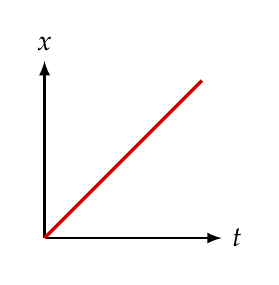
\begin{tikzpicture}[scale=.5]
      \draw[->,thick] (0,0)--(4.5,0) node[right]{$t$};
      \draw[->,thick] (0,0)--(0,4.5) node[above]{$x$};
      \draw[red!80!black,very thick](0,0)--(4,4);
    \end{tikzpicture}
    \hspace{.15in}
    \begin{tikzpicture}[scale=.5]
      \draw[->,thick] (0,0)--(4.5,0) node[right]{$t$};
      \draw[->,thick] (0,0)--(0,4.5) node[above]{$v$};
      \draw[red!80!black,very thick](0,2)--(4,2);
    \end{tikzpicture}
    \hspace{.15in}
    \begin{tikzpicture}[scale=.5]
      \draw[->,thick] (0,0)--(4.5,0) node[right]{$t$};
      \draw[->,thick] (0,0)--(0,4.5) node[above]{$a$};
      \draw[red!80!black,very thick](0,0)--(4,0);
    \end{tikzpicture}
  \end{center}
  \begin{itemize}
  \item Constant velocity has a straight line in the $x-t$ graph
  \item The slope of the $x-t$ graph is the velocity $v$, which is constant
  \item The slope of the $v-t$ graph is the acceleration $a$, which is zero in
    this case
  \end{itemize}
\end{frame}



\begin{frame}{Uniform Acceleration: Constant Acceleration}
  \begin{center}
    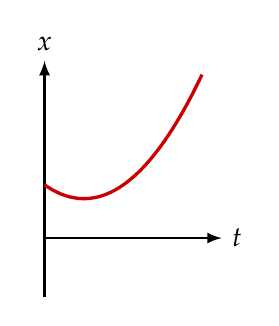
\begin{tikzpicture}[scale=.5]
      \draw[->,thick] (0,0)--(4.5,0) node[right]{$t$};
      \draw[->,thick] (0,-1.5)--(0,4.5) node[above]{$x$};
      \draw[smooth,samples=20,domain=0:4,red!80!black,very thick]
      plot({\x},{0.35*(\x-1)*(\x-1)+1});
    \end{tikzpicture}
    \hspace{.15in}
    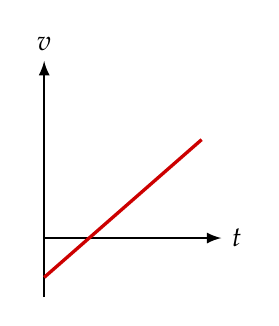
\begin{tikzpicture}[scale=.5]
      \draw[->,thick] (0,0)--(4.5,0) node[right]{$t$};
      \draw[->,thick] (0,-1.5)--(0,4.5) node[above]{$v$};
      \draw[red!80!black,very thick](0,-1)--(4,2.5);
    \end{tikzpicture}
    \hspace{.15in}
    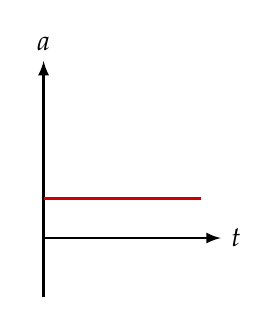
\begin{tikzpicture}[scale=.5]
      \draw[->,thick] (0,0)--(4.5,0) node[right]{$t$};
      \draw[->,thick] (0,-1.5)--(0,4.5) node[above]{$a$};
      \draw[red!80!black,very thick](0,1)--(4,1);
    \end{tikzpicture}
  \end{center}
  \begin{itemize}
  \item The $x-t$ graph for motion with constant acceleration is part of a
    \emph{parabola}
    \begin{itemize}
    \item If the parabola opens up, then acceleration is positive
    \item If the parabola opens down, then acceleration is negative
    \end{itemize}
  \item The $v-t$ graph is a straight line; its slope (a constant) is the
    acceleration
  \end{itemize}
\end{frame}



\begin{frame}{Simple Harmonic Motion}
  For \textbf{harmonic motions}, neither position, velocity nor acceleration
  are constant:

  \vspace{-.1in}
  \begin{center}
    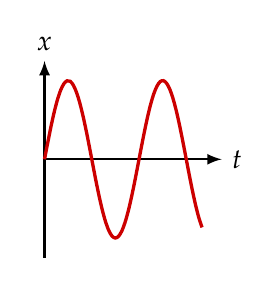
\begin{tikzpicture}[scale=.5]
      \draw[->,thick] (0,0)--(4.5,0) node[right]{$t$};
      \draw[->,thick] (0,-2.5)--(0,2.5) node[above]{$x$};
      \draw[smooth,samples=50,domain=0:4,red!80!black,very thick]
      plot({\x},{2*sin(150*\x)});
    \end{tikzpicture}
    \hspace{.15in}
    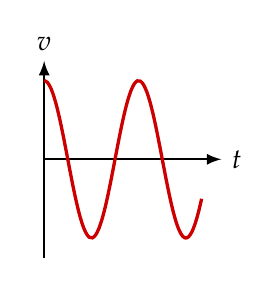
\begin{tikzpicture}[scale=.5]
      \draw[->,thick] (0,0)--(4.5,0) node[right]{$t$};
      \draw[->,thick] (0,-2.5)--(0,2.5) node[above]{$v$};
      \draw[smooth,samples=50,domain=0:4,red!80!black,very thick]
      plot({\x},{2*cos(150*\x)});
    \end{tikzpicture}
    \hspace{.15in}
    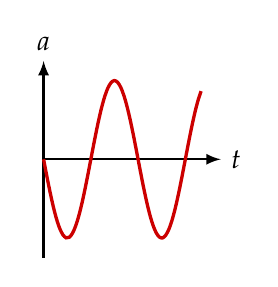
\begin{tikzpicture}[scale=.5]
      \draw[->,thick] (0,0)--(4.5,0) node[right]{$t$};
      \draw[->,thick] (0,-2.5)--(0,2.5) node[above]{$a$};
      \draw[smooth,samples=50,domain=0:4,red!80!black,very thick]
      plot({\x},{-2*sin(150*\x)});
    \end{tikzpicture}
  \end{center}
  Bottom line: regardless of the type motion,
  \begin{itemize}
  \item The $v-t$ graph is the slope of the $x-t$ graph
  \item The $a-t$ graph is the slope of the $v-t$ graph
  \end{itemize}
\end{frame}



\begin{frame}{Area Under Motion Graphs}
  \begin{columns}
    \column{.25\textwidth}
    \begin{center}
      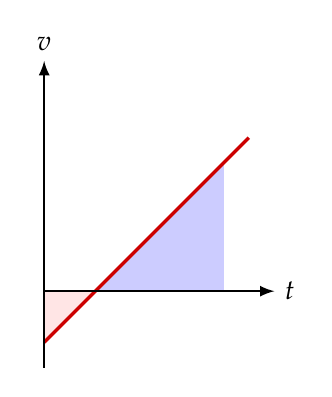
\begin{tikzpicture}[scale=.65]
        \draw[pink!40,fill=pink!40](0,0)--(0,-1)--(1,0)--cycle;
        \draw[blue!20,fill=blue!20](1,0)--(3.5,0)--(3.5,2.5)--cycle;
        \draw[red!80!black,very thick](0,-1)--(4,3);
        \draw[->,thick] (0,0)--(4.5,0) node[right]{$t$};
        \draw[->,thick] (0,-1.5)--(0,4.5) node[above]{$v$};
      \end{tikzpicture}
    \end{center}
    
    \column{.75\textwidth}
    The area under the $v-t$ graph is the displacement $x-x_0$.
    \begin{itemize}
    \item Area \textcolor{blue!20}{\emph{above}} the time axis: $+$
      displacement
    \item Area \textcolor{red!40}{\emph{below}} the time axis: $-$ displacement
    \end{itemize}
    \vspace{.2in}Likewise, the area under the $a-t$ graph is the change in
    velocity $v-v_0$.
  \end{columns}
\end{frame}



\begin{frame}{Velocity Squared vs.\ Displacement}
  If velocity information is given as a function of position\footnote{Depends
    on experimental set up} then a motion graph can be plotted using this
  kinematic equation:

  \eq{-.2in}{
    \underbracket{v^2}_y=\underbracket{v_0^2}_b+\underbracket{2a}_m
    \underbracket{(x-x_0)}_x
  }

  by plotting $v^2$ on the $y$-axis and displacement $\Delta x=x-x_0$ on the
  $x$-axis. The slope of the graph is $m=2a$. The square of the initial
  velocity ($v_0^2$) is the $y$-intercept.
\end{frame}



\begin{frame}{Graphing ``Linear'' Functions}
  This concept extends to graphing other physical quantities not relating to
  motion:
  
  \vspace{.1in}
  \begin{itemize}
  \item To find the index of refraction of a material using Snell's law, plot
    $\sin\theta_i$ vs.\ $\sin\theta_2$ (rather than $\theta_1$ vs.\ $\theta_2$).
    The slope is the index $n$:

    \eq{-.25in}{
      \underbracket{\sin\theta_1}_y=\underbracket{n}_m
      \underbracket{\sin\theta_2}_x
    }
  \item To relate the period of oscillation of a simple pendulum to the length
    of the pendulum, plot $T^2$ vs.\ $L$:

    \eq{-.2in}{
      \underbracket{T^2}_y=\underbracket{\frac{4\pi^2}{g}}_m
      \underbracket{L}_x
    }
  \end{itemize}
\end{frame}


\section{Projectile Motion}

\begin{frame}{Projectile Motion}
  A \textbf{projectile} is an object that is launched with an initial velocity
  of $\bm{v}_0$ along a parabolic trajectory and accelerates only due to
  gravity.
  \begin{center}
    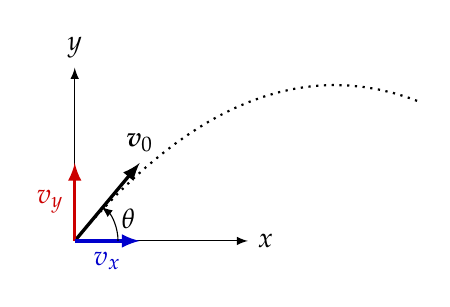
\begin{tikzpicture}[scale=1.1]
      \draw[->](0,0)--(2,0) node[right]{$x$};
      \draw[->](0,0)--(0,2) node[above]{$y$};
      \draw[dotted,domain=0:4,thick] plot (\x, {1.2*\x-.2*\x*\x});
      \draw[very thick,->](0,0)--(.75,.9)node[above]{$\bm{v}_0$};
      \draw[very thick,red!80!black,->]
      (0,0)--(0,.9)node[midway,left]{$v_y$};
      \draw[very thick,blue!80!black,->]
      (0,0)--(.75,0)node[midway,below]{$v_x$};
      \draw[->](.5,0)arc(0:52:.5) node[pos=.6,right]{$\theta$};
    \end{tikzpicture}
  \end{center}
  \begin{itemize}
  \item $x$-axis is the \emph{horizontal} direction, with the ($+$) direction
    pointing \emph{forward}
  \item $y$-axis is the \emph{vertical} direction, with the ($+$) direction
    pointing \emph{up}
  \item The reference point is where the projectile is launched
  \item Consistent with the right-handed Cartesian coordinate system
  \item The launch angle $\theta$ is measured above the the horizontal.
  \end{itemize}
\end{frame}



\begin{frame}{Horizontal ($x$) Direction}
  There is no acceleration (i.e.\ $a_x=\num{0}$) along the horizontal direction,
  therefore horizontal velocity is constant. The kinematic equations reduce to:

  \eq{-.2in}{
    x(t)=v_xt=\left[v_0\cos\theta\right] t
  }

  where $x(t)$ is the horizontal position at time $t$, $v_0$ is the
  magnitude of the initial velocity, $v_x=v_0\cos\theta$ is its horizontal
  component.
\end{frame}




\begin{frame}{Vertical ($y$) Direction}
  Constant acceleration due to gravity alone along the vertical direction, i.e.\
  $a_y=-g$. (Acceleration is \emph{negative} due to the way we defined the
  coordinate system.) The important equation is this one:

  \eq{-.2in}{
    y(t) = \left[v_0\sin\theta\right]t-\frac12gt^2
  }

  These two kinematic equations may also be useful:

  \vspace{-.2in}{\Large
    \begin{align*}
      v_y &= \left[v_0\sin\theta\right] -gt\\
      v_y^2&=\left[v_0\sin\theta\right]^2-2gy
    \end{align*}
  }
\end{frame}



\begin{frame}{Solving Projectile Motion Problems}
  Horizontal and vertical motions are independent of each other, but there are
  variables that are shared in both directions, namely:
  \begin{itemize}
  \item Time $t$
  \item Launch angle $\theta$ (above the horizontal)
  \item Initial speed $v_0$
  \end{itemize}
  
  \vspace{.2in}When solving any projectile motion problems
  \begin{itemize}
  \item \emph{Two} equations with \emph{two} unknowns
  \item If an object lands on an incline, there will be a third equation
    describing the relationship between $x$ and $y$
  \end{itemize}
\end{frame}



\begin{frame}{Symmetric Trajectory}
  A projectile's trajectory is symmetric if the object lands at the same height
  as when it launched. These equations are \emph{not} provided in the AP Exam
  equation sheet, but it can save you a lot of time if you can use them, instead
  of deriving them during the exam.
  \begin{itemize}
  \item Time of flight
    \eq{-.1in}{T=\frac{2v_0\sin\theta}{g}}
  \item Range
    \eq{-.1in}{R=\frac{v_0^2\sin(2\theta)}{g}}
  \item Maximum height
    \eq{-.1in}{H=\frac{v_0^2\sin^2\theta}{2g}}
  \end{itemize}
\end{frame}



\begin{frame}{Maximum Range}
  \eq{-.1in}{
    R=\frac{v_0^2\sin(2\theta)}g
  }
  
  \begin{itemize}
  \item Maximum range occurs at $\displaystyle\theta=\ang{45}$
  \item For a given initial speed $v_0$ and range $R$, launch angle $\theta$ is
    given by:
    
    \eq{-.2in}{
      \theta_1=\frac{1}{2}\sin^{-1}\left(\frac{Rg}{v_0^2}\right)
    }

    But there is another angle that \emph{gives the same range}!

    \eq{-.2in}{
      \theta_2=\ang{90}-\theta_1
    }
  \end{itemize}
\end{frame}



\section{Relative Motion}

\begin{frame}{Relative Motion}
  
  \begin{block}{}
    \textbf{All motion quantities must be measured relative to a
      \emph{frame of reference}}
  \end{block}

  \vspace{.2in}
  \begin{itemize}
  \item\textbf{Frame of reference:} the \emph{coordinate system} from which all
    physical measurements are made.
  \item In \emph{classical} mechanics, the coordinate system is the
    Cartesian system
  \item There is no absolute motion/rest: all motions are relative
  \item\textbf{Principle of Relativity:} All laws of physics are equal in all
    inertial (non-accelerating) frames of reference
  \end{itemize}
\end{frame}  



\begin{frame}{Relative Motion}
  \begin{columns}
    \column{.4\textwidth}
    \begin{tikzpicture}[scale=1.3]
      \draw[->](0,0)--(-.5,-.5) node[left]{$x'$}
      node[pos=0,above left]{$C$};
      \draw[->](0,0)--(1,0)     node[right]{$y'$};
      \draw[->](0,0)--(0,1)     node[above]{$z'$};

      \draw[->](2,3)--(1.5,2.5) node[left]{$x$}
      node[pos=0,above left]{$B$};
      \draw[->](2,3)--(3,3)     node[right]{$y$};
      \draw[->](2,3)--(2,4)     node[above]{$z$};

      \fill[red!70!black] (3,1) circle(.03) node[below right]{$A$};
    \end{tikzpicture}

    \column{.6\textwidth}
    Two frames of reference
    \begin{itemize}
    \item $B$ with axes $x,y,z$
    \item $C$ with axes $x',y',z'$
    \end{itemize}
    The two reference frames may (or may not) be moving relative to each other.
    The motion of the two reference frames affect how motion of
    $\textcolor{red!70!black}{A}$ is calculated.
  \end{columns}
\end{frame}


\begin{frame}{Relative Motion}
  \begin{columns}
    \column{.4\textwidth}
    \begin{tikzpicture}[scale=1.3]
      \draw[->](0,0)--(-.5,-.5) node[left]{$x'$}
      node[pos=0,above left]{$C$};
      \draw[->](0,0)--(1,0)     node[right]{$y'$};
      \draw[->](0,0)--(0,1)     node[above]{$z'$};

      \draw[->](2,3)--(1.5,2.5) node[left]{$x$}
      node[pos=0,above left]{$B$};
      \draw[->](2,3)--(3,3)     node[right]{$y$};
      \draw[->](2,3)--(2,4)     node[above]{$z$};

      \fill[red!70!black] (3,1) circle(.03) node[below right]{$A$};
      \draw[very thick,->,blue!70!black](0,0)--(2.98,.998)
      node[midway,below]{$\bm{x}_{AC}$};
      \draw[very thick,->,green!80!black](2,3)--(3,1.03)
      node[midway,right]{$\bm{x}_{AB}$};
    \end{tikzpicture}

    \column{.6\textwidth}
    The position of $\textcolor{red!70!black}{A}$ can be described by
    \begin{itemize}
    \item $\textcolor{green!80!black}{\bm{x}_{AB}(t)}$ (relative to frame $B$)
    \item $\textcolor{blue!70!black}{\bm{x}_{AC}(t)}$ (relative to frame $C$)
    \end{itemize}
    It is obvious that $\textcolor{green!80!black}{\bm{x}_{AB}(t)}$ and
    $\textcolor{blue!70!black}{\bm{x}_{AC}(t)}$ are different vectors
  \end{columns}
\end{frame}



\begin{frame}{Relative Motion}
  \begin{columns}
    \column{.4\textwidth}
    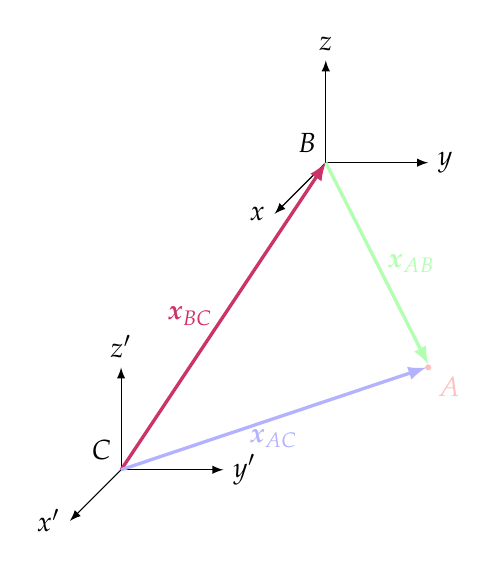
\begin{tikzpicture}[scale=1.3]
      \draw[->](0,0)--(-.5,-.5) node[left]{$x'$}
      node[pos=0,above left]{$C$};
      \draw[->](0,0)--(1,0)     node[right]{$y'$};
      \draw[->](0,0)--(0,1)     node[above]{$z'$};

      \draw[->](2,3)--(1.5,2.5) node[left]{$x$}
      node[pos=0,above left]{$B$};
      \draw[->](2,3)--(3,3)     node[right]{$y$};
      \draw[->](2,3)--(2,4)     node[above]{$z$};
      
      \draw[very thick,->,purple!80](0,0)--(2,3)
      node[midway,left]{$\bm{x}_{BC}$};
      \fill[pink] (3,1) circle(.03) node[below right]{$A$};
      \draw[very thick,->,blue!30](0,0)--(2.98,.998)
      node[midway,below]{$\bm{x}_{AC}$};
      \draw[very thick,->,green!30](2,3)--(3,1.03)
      node[midway,right]{$\bm{x}_{AB}$};
    \end{tikzpicture}

    \column{.6\textwidth}
    The position vector of the origins of the two reference frames is given by
    $\textcolor{purple!80}{\bm{x}_{BC}}$
    \begin{itemize}
    \item The vector pointing from the origin of frame $C$ to the origin of
      frame $B$
    \item If the two frames are moving relative to each other, then
    $\textcolor{purple!80}{\bm{x}_{BC}}$ is also a function of time
    \end{itemize}
    Even without using vector notations, the relationship between the vectors
    is obvious:

    \eq{-.3in}{
      \boxed{
        \textcolor{blue!70!black}{\bm{x}_{AC}}=
        \textcolor{green!80!black}{\bm{x}_{AB}}+
        \textcolor{purple!80}{\bm{x}_{BC}}
      }
    }
  \end{columns}
\end{frame}



\begin{frame}{Relative Motion}
  \begin{columns}
    \column{.4\textwidth}
    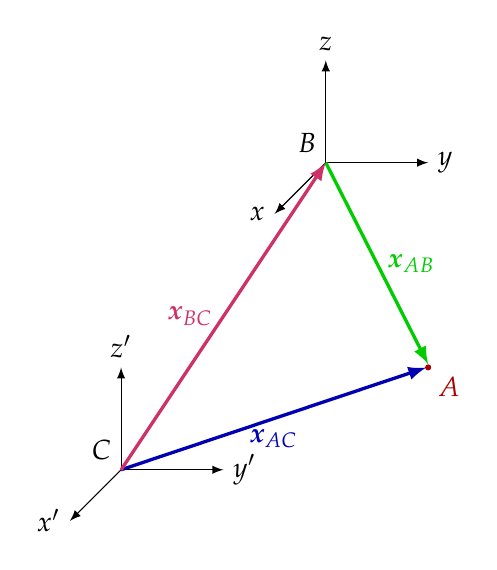
\begin{tikzpicture}[scale=1.3]
      \draw[->](0,0)--(-.5,-.5)  node[left]{$x'$}
      node[pos=0,above left]{$C$};
      \draw[->](0,0)--(1,0) node[right]{$y'$};
      \draw[->](0,0)--(0,1) node[above]{$z'$};

      \draw[->](2,3)--(1.5,2.5)
      node[left]{$x$}
      node[pos=0,above left]{$B$};
      \draw[->](2,3)--(3,3) node[right]{$y$};
      \draw[->](2,3)--(2,4) node[above]{$z$};

      \fill[red!65!black] (3,1) circle(.03) node[below right]{$A$};
      \draw[very thick,->,blue!70!black](0,0)--(2.98,.998)
      node[midway,below]{$\bm{x}_{AC}$};
      \draw[very thick,->,green!80!black](2,3)--(3,1.03)
      node[midway,right]{$\bm{x}_{AB}$};
      \draw[very thick,->,purple!80](0,0)--(2,3)
      node[midway,left]{$\bm{x}_{BC}$};
    \end{tikzpicture}

    \column{.6\textwidth}
    Starting from the definition of \textbf{relative position}:

    \eq{-.33in}{
      \boxed{
        \textcolor{blue!70!black}{\bm{x}_{AC}}=
        \textcolor{green!80!black}{\bm{x}_{AB}}+
        \textcolor{purple!80}{\bm{x}_{BC}}
      }
    }
    
    \vspace{-.1in}Differentiating all terms with respect to time, we get the
    equation for \textbf{relative velocity}:

    \eq{-.25in}{
      \boxed{
        \textcolor{blue!70!black}{\bm{v}_{AC}} =
        \textcolor{green!80!black}{\bm{v}_{AB}}+
        \textcolor{purple!80}{\bm{v}_{BC}}
      }
    }

    \vspace{-.1in}Differentiating with respect to time again, and we obtain
    the equation for \textbf{relative acceleration}:

    \eq{-.25in}{
      \boxed{
        \textcolor{blue!70!black}{\bm{a}_{AC}}=
        \textcolor{green!80!black}{\bm{a}_{AB}}+
        \textcolor{purple!80}{\bm{a}_{BC}}
      }
    }
  \end{columns}
\end{frame}



\begin{frame}{Relative Velocity}
  In classical mechanics, the equation for relative velocities follows the
  \textbf{Galilean velocity addition rule}, which applies to speeds much less
  than the speed of light:

  \eq{-.25in}{
    \bm{v}_{AC}=\bm{v}_{AB}+\bm{v}_{BC}
  }

  The velocity of $A$ relative to reference frame $C$ is the velocity of $A$
  relative to reference frame $B$, plus the velocity of $B$ relative to $C$. If
  we add another reference frame $D$, the equation becomes:

  \eq{-.25in}{
    \bm{v}_{AD}=\bm{v}_{AB}+\bm{v}_{BC}+\bm{v}_{CD}
  }
\end{frame}



\begin{frame}{Typical Problems}
  In an AP Physics C exam, questions involving only kinematics usually appear
  in the multiple-choice section. The problems themselves are not very different
  compared to the Grade 12 Physics problems, but:
  \begin{itemize}
  \item You have to solve problems faster because of time constraint
  \item You can use $g=\SI{10}{\metre/\second\squared}$
    in your calculations to make your lives simpler
  \item Many problems are \emph{symbolic}, which means that they deal with
    the equations, not actual numbers
  \item Will be coupled with other types (e.g.\ dynamics and rotational) in
    the free-response section
  \item You \emph{will} be given an equation sheet
  \end{itemize}
\end{frame}

\end{document}
